\setcounter{tocdepth}{3}
\setcounter{secnumdepth}{3}

\chapter{System Usage}

\section{Communication Server}

The setup enabled the server to start automatically with the Jetson, so after installation be sure to restart your device.

\section{ User Application }
\subsection{Drone list page (main page)}

\subsubsection{Drone(s) offline}
\begin{minipage}[c]{0.5\linewidth}
	\centering
	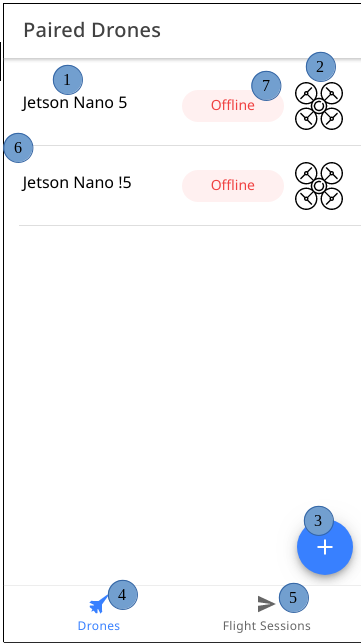
\includegraphics[scale=0.4]{./assets/images/offline.png}
	\label{fig: mainPageOffline}
	\captionof{figure}{Figure 2: Drone list page (with offline drones)}
\end{minipage}
\begin{minipage}[c]{0.5\linewidth}
	\begin{itemize}
		\item (1) Drone name
		\item (2) Drone icon
		\item (3) Navigate to 'add new drone' page
		\item (4) Navigate to drone list page
		\item (5) Navigate to flight sessions page
		\item (6) Drone list
	\end{itemize}
\end{minipage}

\newpage
\subsubsection{Drone(s) online}
\begin{minipage}[c]{0.5\linewidth}
	\centering
	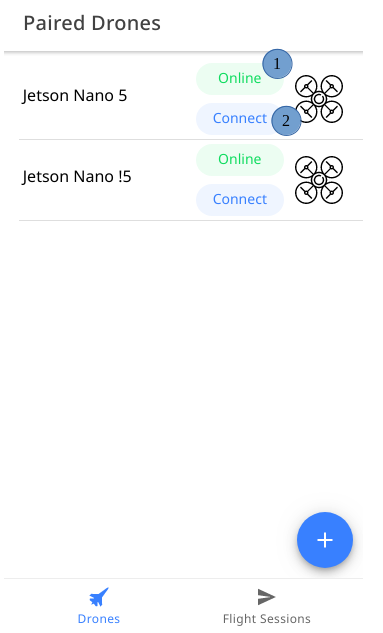
\includegraphics[scale=0.4]{./assets/images/online.png}
	\label{fig: mainPageOnline}
	\captionof{figure}{Figure 3: Drone list page (with online drones)}
\end{minipage}
\begin{minipage}[c]{0.5\linewidth}
	\begin{itemize}
			\item (1) Server status (online)
			\item (2) Connect to drone/server button
	\end{itemize}
\end{minipage}

% \rule{\textwidth}{0.005cm}

\subsubsection{Drone(s) online and connected}
\begin{minipage}[c]{0.5\linewidth}
	\centering
	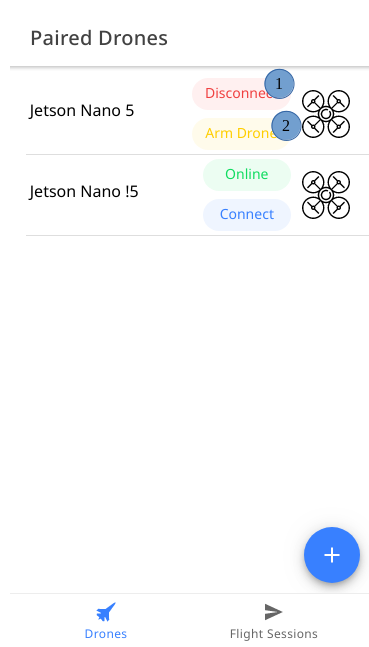
\includegraphics[scale=0.4]{./assets/images/connected.png}
	\label{fig: mainPageConnected}
	\captionof{figure}{Figure 4: Drone list page (with online and connected drones)}
\end{minipage}
\begin{minipage}[c]{0.5\linewidth}
	\begin{itemize}
			\item 1. Disconnect drone button
			\item 2. Arm drone button (which initialises object recognition \cite{darknet} and launches the drone)
	\end{itemize}
\end{minipage}

\newpage
\subsubsection{Drone(s) connected and armed}
\begin{minipage}[c]{0.5\linewidth}
	\centering
	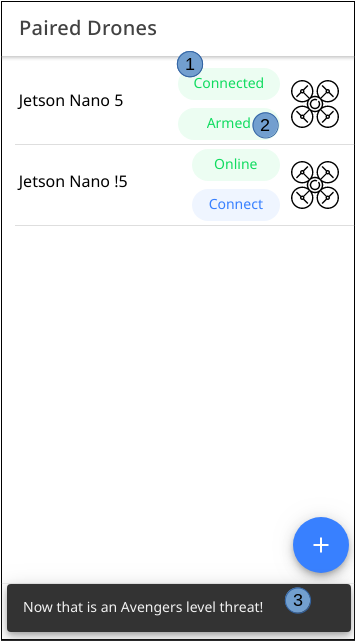
\includegraphics[scale=0.4]{./assets/images/armed.png}
	\label{fig: mainPageArmed}
	\captionof{figure}{Figure 5: Drone list page (with connected and armed drones)}
\end{minipage}
\begin{minipage}[c]{0.5\linewidth}
	\begin{itemize}
		\item (1) Connection status (connected)
		\item (2) Armed status button (currently armed). If this button is clicked, the drone will disarm itself (which turns off object recognition and the drone will proceed to land itself)
		\item (3) Notification alerting user of detection from drone
	\end{itemize}
\end{minipage}

\subsubsection{Delete an existing drone}
\begin{minipage}[c]{0.5\linewidth}
	\centering
	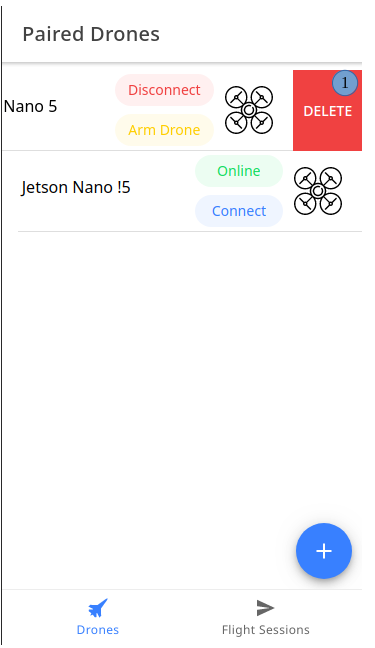
\includegraphics[scale=0.4]{./assets/images/delete.png}
	\label{fig: mainPageDroneDelete}
	\captionof{figure}{Figure 6: Drone list page (with delete action)}
\end{minipage}
\begin{minipage}[c]{0.5\linewidth}
	\begin{itemize}
		\item (1) Delete button (which deletes currently selected drone). This button is reached by swiping from Right -> Left on a specific drone.
	\end{itemize}
\end{minipage}

\newpage
\subsubsection{Modify an existing drone's settings}
\begin{minipage}[c]{0.5\linewidth}
	\centering
	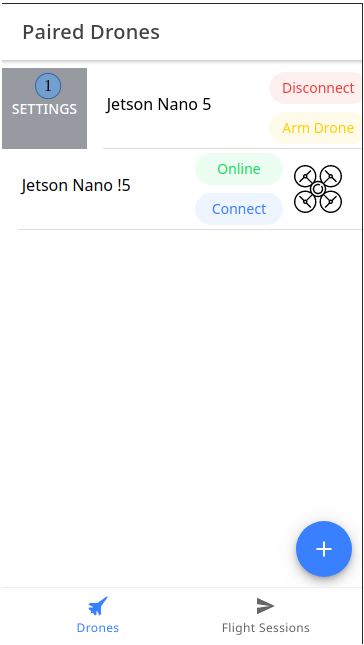
\includegraphics[scale=0.4]{./assets/images/settings.png}
	\label{fig: mainPageDroneSettings}
	\captionof{figure}{Figure 7: Drone list page (with settings action)}
\end{minipage}
\begin{minipage}[c]{0.5\linewidth}
	\begin{itemize}
		\item (1) Settings button (which navigates to the drone settings menu where the currently selected drone's settings can be modified). This button is reached by swiping from Left -> Right on a specific drone.
	\end{itemize}
\end{minipage}

\subsection{Drone settings page}
\subsubsection{Add a new drone or modify an existing drone's settings}
\begin{minipage}[c]{0.5\linewidth}
	\centering
	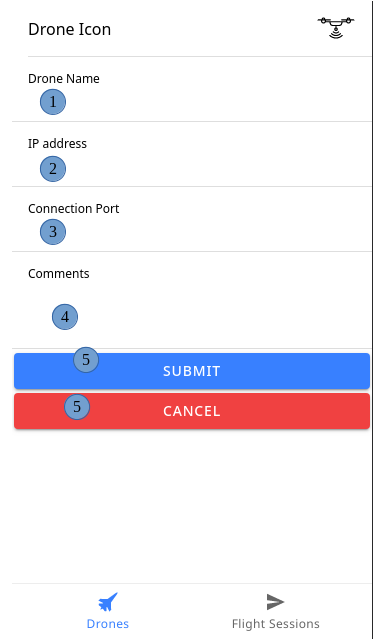
\includegraphics[scale=0.4]{./assets/images/add-new.png}
	\label{fig: settingsPageDroneAdd}
	\captionof{figure}{Figure 8: New drone page}
\end{minipage}
\begin{minipage}[c]{0.5\linewidth}
	\begin{itemize}
		\item (1) Drone name
		\item (2) Drone IP address
		\item (3) Drone connection port
		\item (4) General comments
		\item (5) Submit button
		\item (6) Cancel button (navigate back to drone list page)
	\end{itemize}
\end{minipage}

\newpage
\subsection{Flight sessions page}
\subsubsection{All sessions tab}
\begin{minipage}[c]{0.5\linewidth}
	\centering
	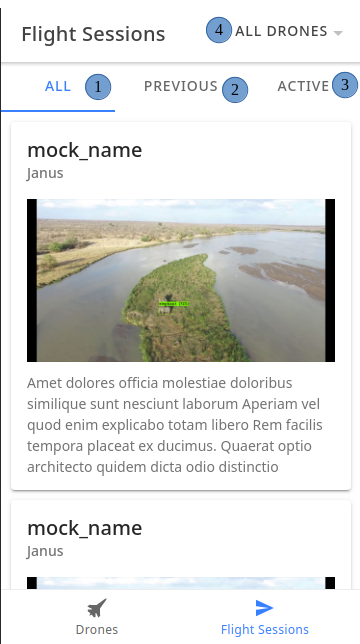
\includegraphics[scale=0.4]{./assets/images/all-sessions.png}
	\label{fig: sessionsPageAll}
	\captionof{figure}{Figure 9: Flight sessions page (with "all sessions" tab selected)}
\end{minipage}
\begin{minipage}[c]{0.5\linewidth}
	\begin{itemize}
		\item (1) Navigates to "all sessions" tab
		\item (2) Navigates to "previous sessions" tab
		\item (3) Navigates to "active sessions" tab
		\item (4) Tappable dropdown list to filter sessions pertaining to a specific drone that exists on the main page 
	\end{itemize}
\end{minipage}

\subsubsection{Active sessions tab}
\begin{minipage}[c]{0.5\linewidth}
	\centering
	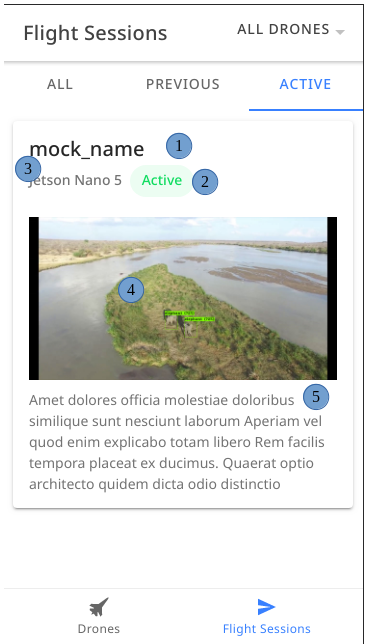
\includegraphics[scale=0.4]{./assets/images/active-sessions.png}
	\label{fig: sessionsPageActive}
	\captionof{figure}{Figure 10: Flight sessions page (with "active sessions" tab selected)}
\end{minipage}
\begin{minipage}[c]{0.5\linewidth}
	\begin{itemize}
		\item (1) Session name
		\item (2) Session status (active)
		\item (3) Drone name (that was active for the specified session)
		\item (4) Image of first detection during the specified session, which came from the drone's video feed
		\item (5) Session description (provided by ranger after ending session)
	\end{itemize}
\end{minipage}

\newpage
\subsubsection{Filter sessions dropdown}
\begin{minipage}[c]{0.5\linewidth}
	\centering
	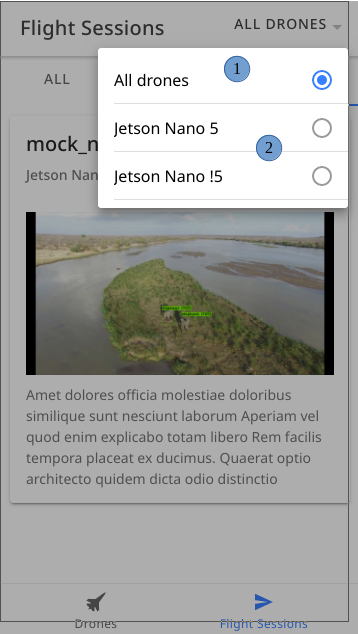
\includegraphics[scale=0.4]{./assets/images/filter.png}
	\label{fig: sessionsPageFilter}
	\captionof{figure}{Figure 11: Flight sessions page (with session filter dropdown tapped)}
\end{minipage}
\begin{minipage}[c]{0.5\linewidth}
	\begin{itemize}
		\item (1) All drones option (which does not apply a filter and consequently displays all sessions from all drones)
		\item (2) Option to choose a specific drone from the list. Filter will then be applied and only sessions pertaining to the selected drone name will be displayed.
	\end{itemize}
\end{minipage}

